\documentclass[11pt]{article}

\usepackage{sectsty}
\usepackage{graphicx}
\graphicspath{{./images/}}

\topmargin=-0.45in
\evensidemargin=0in
\oddsidemargin=0in
\textwidth=6.5in
\textheight=9.0in
\headsep=0.25in

\title{Collaboration between human and AI in typography}
\author{Theodor Peifer}
\date{\today}

\begin{document}
\maketitle	
\pagebreak

\section{INTRODUCTION}
Recent advances in the field of image generation using Artificial Intelligence allow individuals to create stunning images without any creative effort - including in the field of typography.
However, the use of generative AI in arts raises interesting questions about the role of the human in the creative process. On the one hand, the human is taking a passive role, simply providing the input data and allowing the AI to generate the final product. On the other hand, the human is actively participating in the design process: First by designing the AI itself, which requires a big amount of creative thought and effort and secondly by exploring and refining the results the model generated.
This process can be described as "meta-creativity," where the individual only passively participates in the creative work, but instead actively invents creative ways to automate it.
In order to explore and reflect on this concept, I developed an AI which generates new font styles, which will be displayed in a typographic manual. This article will contain a detailed documentation of my process.


\section{METHODOLOGY}
This project consists of three parts: Researching previous work about artifical font generation, developing the model and designing the typographic manual.
The research is done by searching and examining existing papers and their proposed methods. After determining the appropriate model for this problem, the next step is to gather the dataset. Then the model can be built and trained using Python and the Pytorch framework. The best results will be gathered and displayed in the manual, which has to be designed next.


\section{PREVIOUS WORK}
The state-of-the-art model for generating novel type faces has been developed by Hayiashi et al. in their paper \emph{GlyphGAN: Style-Consistent Font Generation Based on Generative Adversarial Networks}. They propose the usage of a \emph{Generative Adversarial Network} (GAN). A GAN consists of two neural networks. The generator and the discriminator. The generator learns to generate "fake" data from random noise and the discriminator network learns to classify between such fake data and real data. The goal of the generator is therefore to fool the discriminator by creating rsynthetic but realistic data. This model can easily be applied to generate fonts and will learn to produce 64x64 black and white images containing a single letter. In order to generate all letters in the alphabet in the same font style, the authors inroduce style-consistency: Instead of feeding the generator just random noise, the input will consist two concantinated vectors: A random style-vector and a vector which numerically represents a letter using one-hot encoding. To produce an alphabet with the same style over all letters, the style-vector has to be the same.
Similar work has been done by Erik Bernhardsson who developed the \emph{deep-fonts} font generator which used a simple dense neural network instead of a convolution based model.
In a detailed comparison by Hayiashi et al. proved that their method produces more consistent and legible glyphs. Therefore this project employs a model heavily influenced by the \emph{GlyphGAN}.


\begin{figure}
    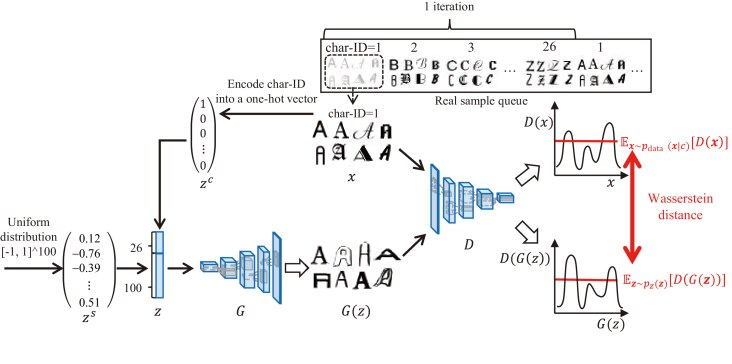
\includegraphics[width=\linewidth]{glyphgan.png}
    \caption{The GlypGAN archtecture.}
    \label{fig:glyphgan}
\end{figure}


\section{DEVELOPMENT OF THE GENERATIVE MODEL}
Since the dataset used to train the \emph{GlyphGAN} is not accessible, the model will be trained using the dataset collected by Bernhardsson for his \emph{deep-fonts} model which consists of 56443 different fonts scraped from the internet. Each font set consists of 62 characters, but for simplicity and better results the model will only be trained on upper-case letters and will therefore be able to create onyl such. When examining random samples of the dataset it becomes obvious that there is a lot of noise present. Noise in this case meaning handwritten "fonts" and even unreadable ones which are expected to reduce the quality of the generated images. Yet, because of time and complexity the dataset has not been cleaned.
The model was developed using the popular and powerful \emph{PyTorch} Deep Learning Framework for Python, which enables the implementation of complex architectures.
This stage of the project took around two weeks, since training a model took up to 5 hours and multiple training runs in order to find the optimal parameters. Although the final model wasn't able to reproduce as good results as shown in the GlyphGAN paper the generated letters still had consistent font styles which could be used a inspiration for typographers.

\section{DESIGN OF THE TYPOGRAPHIC MANUAL}
Designing the typographic manual turned out to be a challenging task for multiple reasons: First, the letters generated by the AI are in a low resolution pixel and not in a vector format which is needed to be usable as a real font. Also, the letters are not pixel perfect, which means that there is often noise around the letter.
Lastly, many glpyhs are not legible or look like other letters in the alphabet (eg. the model is barely able to produce the letter \emph{A} or \emph{S}).

\pagebreak
\section{CONCLUSION}
Lorem Ipsum \\

\end{document}